\subsection{Continuous granularity queries reveal tissue context dependence}
\label{sec:context-zoom}
\label{sec:objective-ablation}
\label{sec:anatomical-scale-preference}
\label{sec:granularity-transfer}
\label{sec:scale-continuum}
\label{sec:context-response}
\raggedbottom

We next examine how tissue descriptions depend on observation granularity, and whether the
learned transformations make this dependence predictable and useful for tissue analysis.

Granularity preferences are related to anatomical structure.
Across annotated regions in the eight held-out MOSTA sections, the
relative advantage of coarse over fine Spatial representations,
measured by regional IoU, increases with neighborhood homogeneity
and decreases with boundary fraction (Figure~\ref{fig:granularity-preferences}; Appendix~\ref{app:region-scale}).
Broader context thus tends to benefit locally homogeneous regions,
whereas finer context favors regions with frequent anatomical boundaries. The Lung and Smooth muscle example in a training section illustrates
this contrast.
Broader context improves Lung delineation, whereas finer context
better preserves the narrow bands and rings of Smooth muscle
(Figure~\ref{fig:results1-mosta}).
Expanding the observation range therefore changes which structures
are resolved best, rather than uniformly improving anatomical recognition.

\begin{figure}[!htb]
\centering
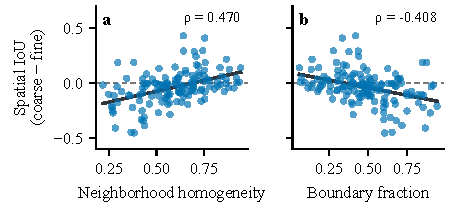
\includegraphics[width=0.55\linewidth]{figures/region_geometry.pdf}
\caption{\textbf{Granularity preferences reflect tissue organization.} Spatial IoU difference ($k=128$ minus $k=8$) versus (a) neighborhood homogeneity and (b) boundary fraction. Solid lines: linear fits; dashed lines: equal IoU. Definitions: Appendix~\ref{app:region-scale}.}
\label{fig:granularity-preferences}
\label{fig:region-geometry}
\end{figure}

These differences motivate asking whether a location's molecular
description at one observation range can predict its description
at another.
On held-out MOSTA sections, we keep the encoder and transformation
frozen and compare predictions with representations encoded directly
from the actual target neighborhoods.
For granularity pairs used during training, predictions are closer
to these references than unchanged source states, with lower mean
MSE on all eight sections (Figure~\ref{fig:granularity-query-summary}a).
Shuffled-pair controls additionally support location-dependent
source--target associations (Appendix~\ref{app:granularity-transfer}).

Prediction also generalizes when both the section and the target
granularity are unseen.
Although trained only at $r \in \{8,32,128\}$, ZoomST predicts
representations at six unseen intermediate granularities from $e_8$,
using target-neighborhood encodings only for evaluation.
Mean target MSE is lower than that of the unchanged source on every
held-out section (Figure~\ref{fig:granularity-query-summary}b; Appendix~\ref{app:unseen-state-detail}).
In a separate comparison with a shared frozen encoder, the ODE
also improves on a granularity-conditioned residual MLP, with a
mean paired reduction of 10.86\% in unseen-granularity MSE
(Appendix~\ref{app:transition-comparison}).

Beyond predicting descriptions at individual granularities, these
queries allow us to ask which locations change more as the observation
range expands.
The predicted response measures representation change per doubling
of context (Equation~\ref{eq:granularity-response}).
Averaged over the tested intervals, locations with high predicted
responses show larger mean changes in directly encoded representations
than those with low predicted responses on all eight held-out sections
(Figure~\ref{fig:granularity-query-summary}c; Appendix~\ref{app:response-meaning}).
This agreement supports comparisons of relative context sensitivity
across locations.

\begin{figure}[!htb]
\centering
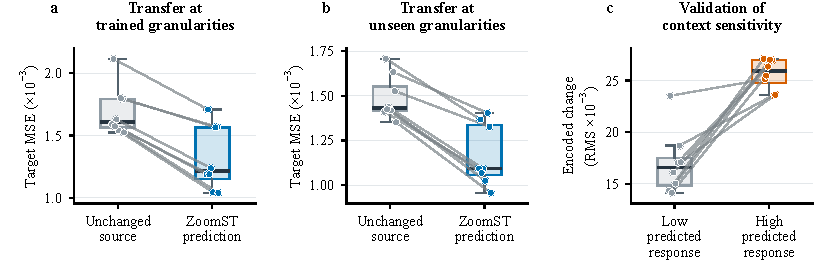
\includegraphics[width=0.95\linewidth]{figures/granularity_query_summary.pdf}
\caption{\textbf{Zero-shot transfer and context sensitivity on eight held-out sections.} (a,b) Target MSE at trained and unseen granularities. (c) Directly encoded change in the lowest and highest predicted-response quarters. Points are section means; lines connect the same section. Boxes show medians, interquartile ranges and 1.5-IQR whiskers. Protocols: Appendix~\ref{app:scale-continuum}.}
\label{fig:granularity-query-summary}
\label{fig:generalization-summary}
\label{fig:heldout-response-ordering}
\end{figure}

Anatomical cases from training sections help interpret what this
sensitivity reflects.
In Facial nerve, stronger predicted responses over $64 \rightarrow 128$
accompany larger shifts from nerve-dominated neighborhoods toward
surrounding tissue (Figure~\ref{fig:ode-context}a).
By contrast, low-response locations already include substantial
surrounding tissue at the finer range and change less as context
expands (Figure~\ref{fig:facial-nerve-composition}).
In this example, the response reflects the change introduced by
additional context, rather than simply how mixed the initial
neighborhood already is.

Context sensitivity also captures changes within an anatomical
compartment.
In Brain, predicted responses track directly encoded changes over
$8 \rightarrow 16$ even among sampled locations whose neighborhoods
remain entirely Brain-labeled at both granularities (Appendix~\ref{app:response-meaning}).
Thus, molecular context can vary with observation range without
a change in broad anatomical composition.
Whole-section maps further show the spatial variation in path-averaged
response alongside observed neighborhood-composition changes
(Figure~\ref{fig:ode-context}b,c).

Together, these results extend tissue analysis from comparing
descriptions at selected granularities to predicting unseen
intermediate descriptions and characterizing their relative
sensitivity to surrounding context.

\begin{figure}[!htb]
\centering
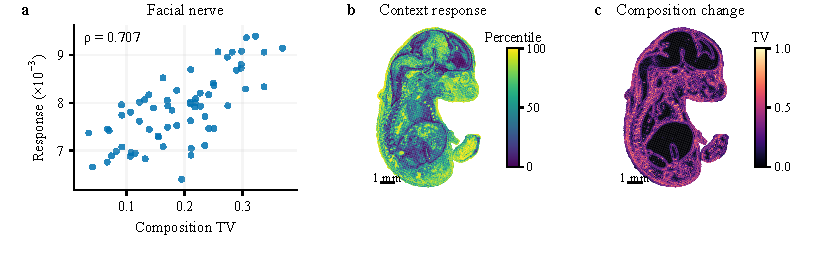
\includegraphics[width=0.95\linewidth]{figures/response_context_overview.pdf}
\caption{\textbf{Anatomical interpretation of context response.} (a) Predicted response versus composition change (total variation; TV) in E14.5 E1S1 Facial nerve ($64\to128$; 64 locations). (b,c) E16.5 E1S1 maps of path-averaged response and composition TV over 8--128. Scale bars: 1\,mm. Definitions and composition-group comparisons: Appendix~\ref{app:response-meaning}.}
\label{fig:ode-context}
\end{figure}
